\documentclass[conference]{IEEEtran}
\IEEEoverridecommandlockouts
% The preceding line is only needed to identify funding in the first footnote. If that is unneeded, please comment it out.
\usepackage{cite}
\usepackage{amsmath,amssymb,amsfonts}
\usepackage{algorithmic}
\usepackage{graphicx}
\usepackage{textcomp}
\usepackage{xcolor}
\usepackage[numbers]{natbib}
\usepackage{listings}
\usepackage{lipsum}
\usepackage{multicol}
\usepackage{hyperref}
\usepackage{enumitem}
\usepackage{float}
\usepackage{tabularx}
\usepackage{graphicx}
\usepackage{subcaption}

\newlist{numitemize}{enumerate}{1}
\setlist[numitemize]{label=\arabic*.}

\lstset{
    language=C++,               
    basicstyle=\ttfamily\footnotesize, 
    keywordstyle=\color{blue},  
    commentstyle=\color{green}, 
    stringstyle=\color{red},    
    numberstyle=\tiny\color{gray},
    stepnumber=1,               
    numbersep=10pt,             
    backgroundcolor=\color{white}, 
    showspaces=false,           
    showstringspaces=false,     
    showtabs=false,             
    frame=single,               
    captionpos=b,               
    breaklines=true,            
    breakatwhitespace=false,    
    tabsize=2                   
}
\begin{document}

\title{Informe de Laboratorio: Pruebas sobre el comportamiento de la Memoria Caché}


\author{\IEEEauthorblockN{1\textsuperscript{st} Justo Alfredo Perez Choque}
    \IEEEauthorblockA{\textit{dept. Ciencia de la Computación} \\
        \textit{Universidad Católica San Pablo}\\
        Arequipa, Perú \\
        justo.perez@ucsp.edu.pe}
}



\maketitle




\section{Introducción}
El objetivo de este laboratorio es estudiar el comportamiento de la memoria caché. Se implementaron dos ejercicios, 
primero una comparación de dos variantes de bucles anidados en C++ y en GO, y se compararon sus tiempos de ejecución para 
observar cómo las diferencias en el acceso a la memoria pueden influir en el desempeño. Luego, se analizó la
 eficiencia de dos algoritmos de multiplicación de matrices, uno clásico y otro basado en bloques, evaluando 
 su rendimiento en términos de \textit{cache hits}, \textit{cache misses},
 y la gestión de la localidad espacial y temporal. El repositorio de todo el trabajo se encuentra en el repositorio\cite{repo}.

\section{Implementación}
\subsection{\textbf{Código del libro: Bucles anidados}}

El código utilizado para este experimento consiste en dos funciones (\texttt{test1} y \texttt{test2})
que realizan operaciones similares sobre una matriz \texttt{A} y dos vectores \texttt{x} e \texttt{y}.


La principal diferencia entre \texttt{test1} y \texttt{test2} radica en el orden de los bucles anidados:
\begin{itemize}
    \item  En \texttt{test1}, el bucle externo itera sobre el índice \texttt{i}, mientras que el bucle interno lo hace sobre el índice \texttt{j}.
    \item  En \texttt{test2}, el orden de los bucles se invierte; el bucle externo itera sobre \texttt{j} y el interno sobre \texttt{i}.
\end{itemize}
Ambas funciones realizan la operación:
\[
    y[i] += A[i][j] \times x[j]
\]

\begin{lstlisting}[language=C++]
void test1(double** A, double* x, double* y, int MAX) {
    for (int i = 0; i < MAX; i++)
        for (int j = 0; j < MAX; j++)
            y[i] += A[i][j] * x[j];
}
void test2(double** A, double* x, double* y, int MAX) {
    for (int j = 0; j < MAX; j++)
        for (int i = 0; i < MAX; i++)
            y[i] += A[i][j] * x[j];
}
\end{lstlisting}
\subsection{\textbf{Código Multiplicación Matrices}}
Realicé dos algoritmos para la multiplicación de matrices: la multiplicación clásica utilizando tres bucles anidados y la multiplicación por bloques utilizando seis bucles anidados.
\begin{lstlisting}[language=C++]
void multMatrizClasica(int **m1, int **m2, int **res, int N ){
   
    for(int i = 0; i < N;i++){
        for(int j = 0; j < N; j++){
            for(int k = 0; k < N; k++){
                *(*(res+i)+j) += *(*(m1+i)+k) * *(*(m2+k)+j);
            }
        }
    }
    return;
}


void multMatrizBloque(int **m1, int **m2, int **res, int N , int S){
    for (int ii = 0; ii < N; ii += S) {
        for (int jj = 0;jj < N; jj += S) {
            for (int kk = 0; kk < N; kk += S) {
                for (int i = ii;i < std::min(ii+S,N); ++i) {
                    for (int j = jj;j < std::min(jj+S, N); ++j) {
                        for (int k = kk; k < std::min(kk +S, N);++k) {
                            res[i][j] += m1[i][k]*m2[k][j];
                        }
                    }
                }
            }
        }
    }
}
\end{lstlisting}


\section{Resultados y Analisis}
\subsection{Especificaciones del Procesador}

Las pruebas de rendimiento fueron realizadas en un procesador \textbf{Intel Core i7-10700F}, cuyas especificaciones son las siguientes:

\begin{itemize}
    \item \textbf{Arquitectura:} \texttt{x86\_64} (soporta \textbf{32-bit} y \textbf{64-bit}).
    \item \textbf{Número de núcleos e hilos:} 
    \begin{itemize}
        \item \textbf{Núcleos físicos:} 8
        \item \textbf{Hilos de ejecución:} 16 (\textit{Hyper-Threading} activado)
    \end{itemize}
    \item \textbf{Frecuencias de operación:} 
    \begin{itemize}
        \item \textbf{Frecuencia base:} 2.90 GHz
        \item \textbf{Frecuencia máxima (Turbo Boost):} 4.80 GHz
        \item \textbf{Frecuencia mínima:} 800 MHz (modo de ahorro de energía)
    \end{itemize}
    \item \textbf{Memoria caché:} 
    \begin{itemize}
        \item \textbf{Caché L1:} 
        \begin{itemize}
            \item \textbf{Datos (L1d):} 256 KiB (8 instancias, 32 KiB por núcleo)
            \item \textbf{Instrucciones (L1i):} 256 KiB (8 instancias, 32 KiB por núcleo)
        \end{itemize}
        \item \textbf{Caché L2:} 2 MiB (8 instancias, 256 KiB por núcleo)
        \item \textbf{Caché L3:} 16 MiB (compartida entre todos los núcleos)
    \end{itemize}
    \item \textbf{Virtualización:} Soporte para \texttt{VT-x} (\textit{Intel Virtualization Technology}).
    \item \textbf{Vulnerabilidades y mitigaciones:} 
    \begin{itemize}
        \item \textbf{Spectre v1 y v2:} Mitigado por microcódigo y software.
        \item \textbf{Meltdown:} No afectado.
        \item \textbf{L1TF, MDS, SRBDS, TAA:} No afectado o mitigado.
        \item \textbf{Spec Store Bypass, Retbleed:} Mitigaciones activadas.
    \end{itemize}
\end{itemize}

\subsection{\textbf{Código del libro: Bucles anidados}}

La Tabla \ref{tabla_cpp} y la Tabla \ref{tabla_go} muestran que la primera forma tiene un mejor 
rendimiento que la segunda, especialmente a medida que el tamaño de la matriz aumenta. Esto se debe
principalmente a cómo ambas formas aprovechan la memoria caché. La primera forma tiene un alto número 
de \textit{cache hits} debido a que accede secuencialmente a la memoria por filas, lo que explota la
\textit{localidad espacial} y \textit{temporal}. Esto significa que los datos adyacentes y recientemente 
utilizados están más frecuentemente disponibles en la caché, reduciendo la necesidad de acceder a la memoria principal.

\begin{table}[h!]
    \centering
    \begin{tabularx}{250pt}{|X|X|X|}
        \hline
        \textbf{Valor de MAX} & \textbf{Primera Forma (segundos)} & \textbf{Segunda Forma (segundos)} \\ \hline
        100                   & 4.1969e-05                        & 4.3164e-05                        \\ \hline
        200                   & 0.000173058                       & 0.000200513                       \\ \hline
        400                   & 0.000657152                       & 0.000898779                       \\ \hline
        800                   & 0.00266543                        & 0.00427397                        \\ \hline
        1600                  & 0.010799                          & 0.0286272                         \\ \hline
        3200                  & 0.0436007                         & 0.134383                          \\ \hline
        6400                  & 0.176388                          & 0.566714                          \\ \hline
        12800                 & 0.714516                          & 3.0812                            \\ \hline
        25600                 & 3.40258                           & 17.342                            \\ \hline
    \end{tabularx}
    \caption{Tiempo de ejecución en segundos para las dos formas de bucles anidados en C++.}
    \label{tabla_cpp}
\end{table}

\begin{table}[h!]
    \centering
    \begin{tabularx}{250pt}{|X|X|X|}
        \hline
        \textbf{Valor de MAX} & \textbf{Primera Forma (segundos)} & \textbf{Segunda Forma (segundos)} \\ \hline
        100                   & 0.007778                          & 0.007468                          \\ \hline
        200                   & 0.026658                          & 0.027440                          \\ \hline
        400                   & 0.106350                          & 0.112743                          \\ \hline
        800                   & 0.428597                          & 0.457661                          \\ \hline
        1600                  & 1.715543                          & 1.908691                          \\ \hline
        3200                  & 6.905817                          & 8.143203                          \\ \hline
        6400                  & 28.105395                         & 32.631453                         \\ \hline
        12800                 & 112.481481                        & 132.151404                        \\ \hline
        25600                 & 445.666284                        & 532.672041                        \\ \hline
    \end{tabularx}
    \caption{Tiempo de ejecución en segundos para las dos formas de bucles anidados en Go.}
    \label{tabla_go}
\end{table}

Por otro lado, la segunda forma accede a la matriz por columnas, lo que provoca un mayor
número de \textit{cache misses} porque los elementos de una columna no están contiguamente
almacenados en la memoria. Esto dificulta el aprovechamiento de la \textit{localidad espacial},
resultando en una menor eficiencia en el uso de la caché.

\begin{figure}[H]
    \centering
    \begin{subfigure}{0.45\textwidth}
        \centering
        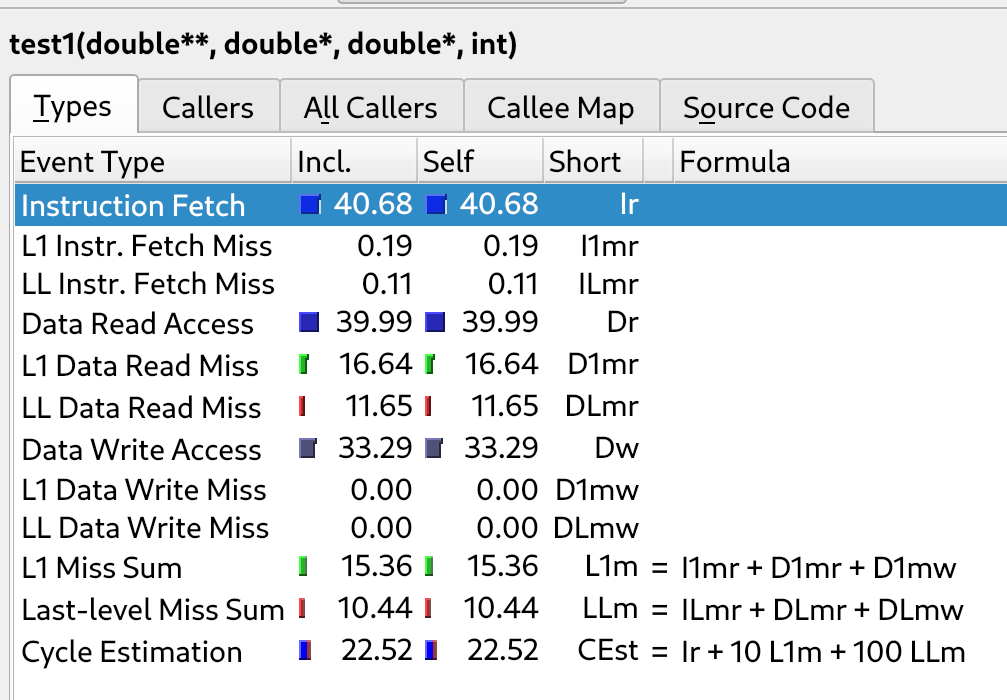
\includegraphics[width=\textwidth]{bucles_cpp_t1.png}
        \caption{Análisis en KCacheGrind - C++ (Test 1)}
    \end{subfigure}
    \hfill
    \begin{subfigure}{0.45\textwidth}
        \centering
        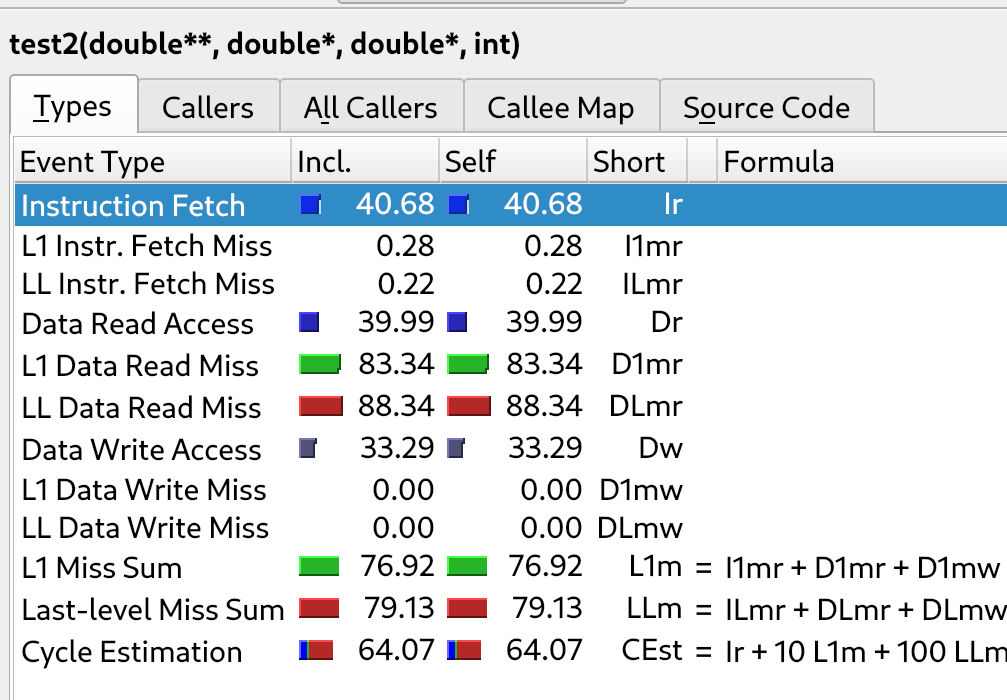
\includegraphics[width=\textwidth]{bucles_cpp_t2.png}
        \caption{Análisis en KCacheGrind - C++ (Test 2)}
    \end{subfigure}

    \begin{subfigure}{0.45\textwidth}
        \centering
        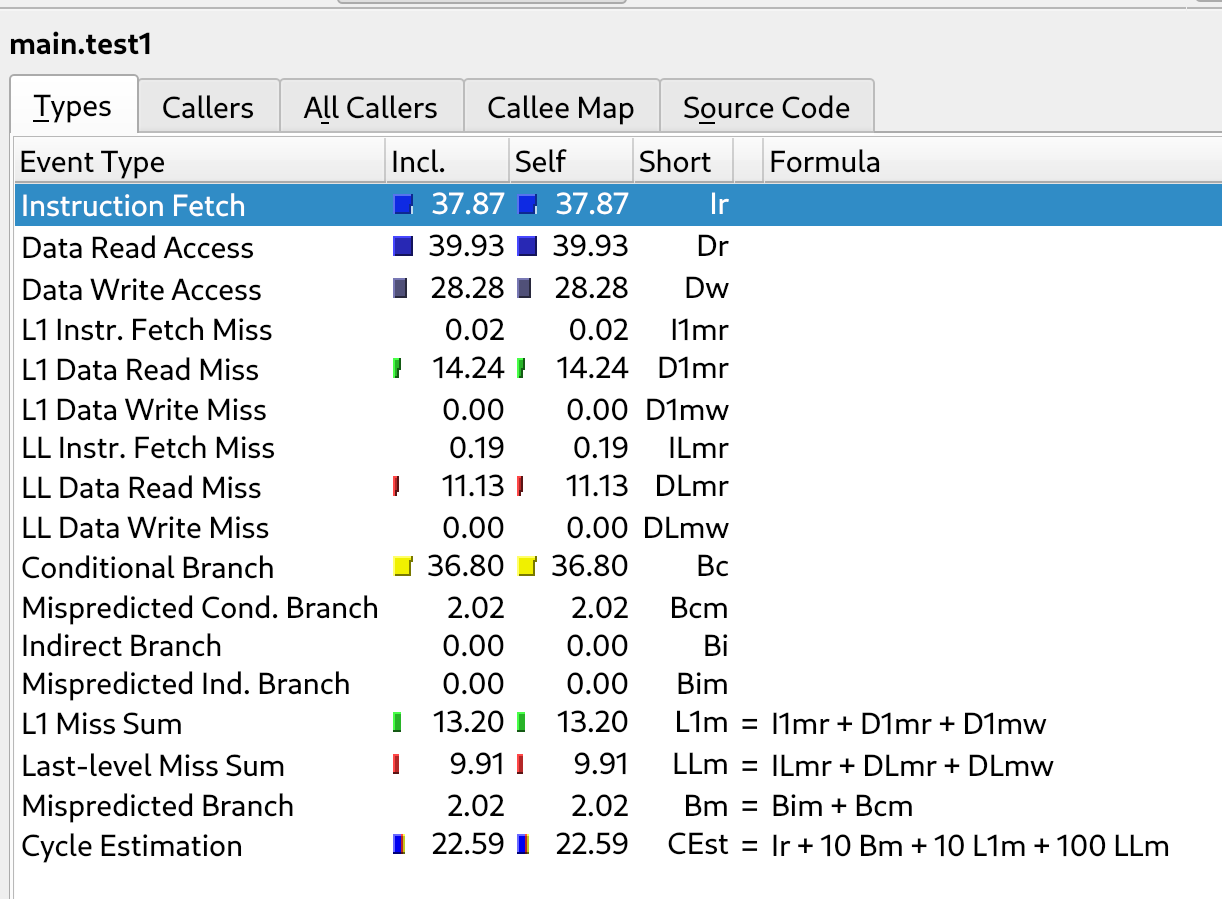
\includegraphics[width=\textwidth]{bucles_go_t1.png}
        \caption{Análisis en KCacheGrind - Go (Test 1)}
    \end{subfigure}
    \hfill
    \begin{subfigure}{0.45\textwidth}
        \centering
        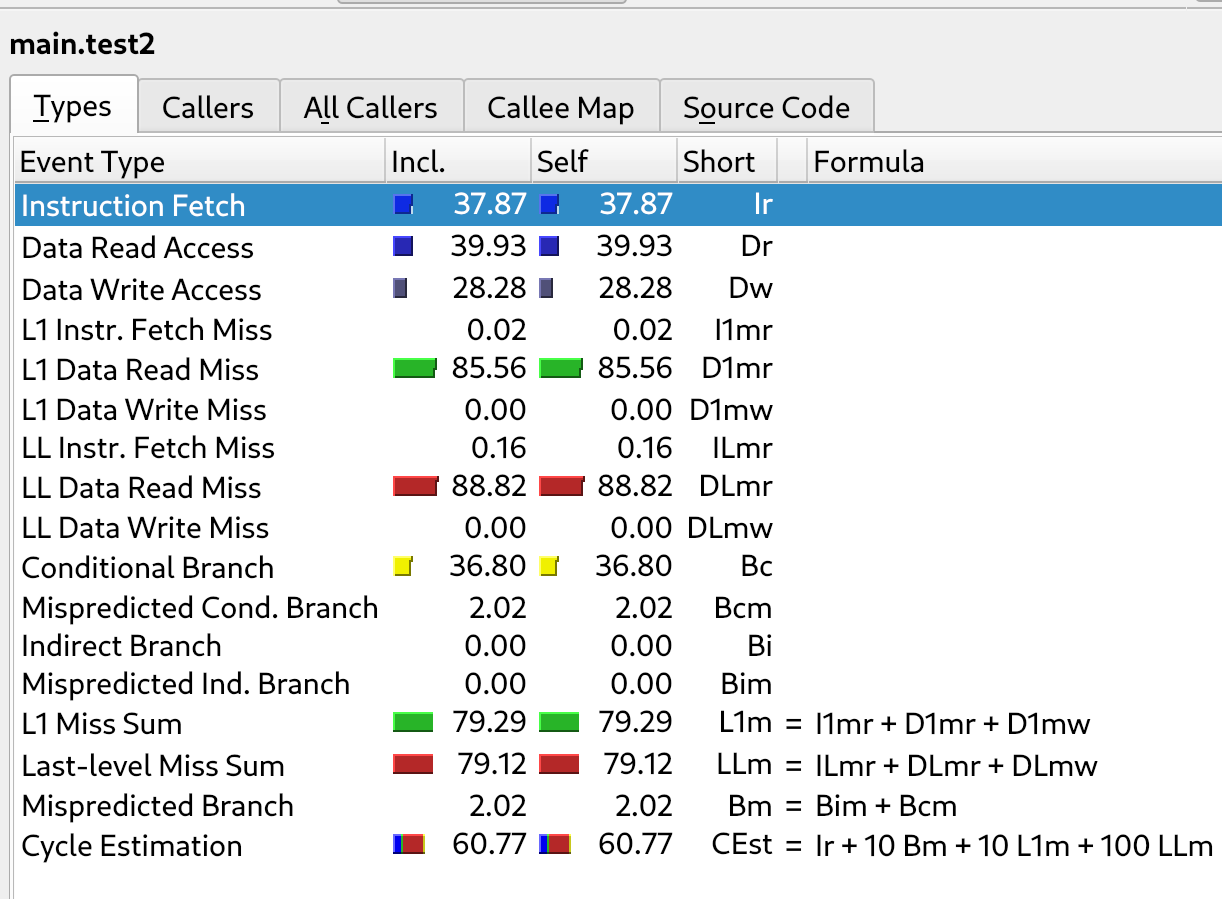
\includegraphics[width=\textwidth]{bucles_go_t2.png}
        \caption{Análisis en KCacheGrind - Go (Test 2)}
    \end{subfigure}

    \caption{Comparación del uso de caché en C++ y Go con KCacheGrind}
    \label{fig:kcachegrind_bucles}
\end{figure}

\subsection{\textbf{Multiplicación de Matrices}}
\subsubsection{\textbf{Analisis y Complejidad}}
La Tabla \ref{Tabla2} muestra una comparación de los tiempos de ejecución para ambos enfoques de multiplicación de matrices.



\begin{table}[h!]
    \centering
    \begin{tabularx}{220pt}{|X|X|X|X|}
    \hline
    \textbf{Tamaño de Matriz} & \textbf{Tamaño de Bloque} & \textbf{Multiplicación Clásica (s)} & \textbf{Multiplicación por Bloques (s)} \\ \hline
    10   & 32  & 0.00131762  & 0.00272606  \\ \hline
    10   & 64  & 0.00131762  & 0.00105588  \\ \hline
    10   & 128 & 0.00131762  & 0.0010516   \\ \hline
    10   & 256 & 0.00131762  & 0.00105044  \\ \hline
    20   & 32  & 0.00379585  & 0.00784878  \\ \hline
    20   & 64  & 0.00379585  & 0.00784101  \\ \hline
    20   & 128 & 0.00379585  & 0.00781941  \\ \hline
    20   & 256 & 0.00379585  & 0.00780592  \\ \hline
    40   & 32  & 0.0304303   & 0.0613677   \\ \hline
    40   & 64  & 0.0304303   & 0.0630941   \\ \hline
    40   & 128 & 0.0304303   & 0.0614604   \\ \hline
    40   & 256 & 0.0304303   & 0.0615096   \\ \hline
    80   & 32  & 0.244707    & 0.47943     \\ \hline
    80   & 64  & 0.244707    & 0.477209    \\ \hline
    80   & 128 & 0.244707    & 0.484576    \\ \hline
    80   & 256 & 0.244707    & 0.486257    \\ \hline
    160  & 32  & 1.96934     & 3.79533     \\ \hline
    160  & 64  & 1.96934     & 3.79366     \\ \hline
    160  & 128 & 1.96934     & 3.77584     \\ \hline
    160  & 256 & 1.96934     & 3.86525     \\ \hline
    320  & 32  & 15.9093     & 30.6567     \\ \hline
    320  & 64  & 15.9093     & 30.1351     \\ \hline
    320  & 128 & 15.9093     & 30.7394     \\ \hline
    320  & 256 & 15.9093     & 30.7268     \\ \hline
    640  & 32  & 129.661     & 242.611     \\ \hline
    640  & 64  & 129.661     & 241.233     \\ \hline
    640  & 128 & 129.661     & 239.914     \\ \hline
    640  & 256 & 129.661     & 246.372     \\ \hline
    1280 & 32  & 1073.4      & 1949.68     \\ \hline
    1280 & 64  & 1073.4      & 2150.53     \\ \hline
    1280 & 128 & 1073.4      & 1908.87     \\ \hline
    1280 & 256 & 1073.4      & 1902.02     \\ \hline
    \end{tabularx}
    \caption{Tiempos de ejecución en segundos en C++.}
    \label{Tabla2}
    \end{table}
    
    \begin{table}[h!]
        \centering
        \begin{tabularx}{220pt}{|X|X|X|X|}
        \hline
        \textbf{Tamaño de Matriz} & \textbf{Tamaño de Bloque} & \textbf{Multiplicación Clásica (s)} & \textbf{Multiplicación por Bloques (s)} \\ \hline
        10   & 32  & 0.00395    & 0.00818    \\ \hline
        10   & 64  & 0.00395    & 0.00317    \\ \hline
        10   & 128 & 0.00395    & 0.00315    \\ \hline
        10   & 256 & 0.00395    & 0.00315    \\ \hline
        20   & 32  & 0.01139    & 0.02354    \\ \hline
        20   & 64  & 0.01139    & 0.02352    \\ \hline
        20   & 128 & 0.01139    & 0.02346    \\ \hline
        20   & 256 & 0.01139    & 0.02342    \\ \hline
        40   & 32  & 0.09129    & 0.18410    \\ \hline
        40   & 64  & 0.09129    & 0.18928    \\ \hline
        40   & 128 & 0.09129    & 0.18438    \\ \hline
        40   & 256 & 0.09129    & 0.18453    \\ \hline
        80   & 32  & 0.73412    & 1.43829    \\ \hline
        80   & 64  & 0.73412    & 1.43163    \\ \hline
        80   & 128 & 0.73412    & 1.45372    \\ \hline
        80   & 256 & 0.73412    & 1.45877    \\ \hline
        160  & 32  & 5.90802    & 11.38599   \\ \hline
        160  & 64  & 5.90802    & 11.38098   \\ \hline
        160  & 128 & 5.90802    & 11.32752   \\ \hline
        160  & 256 & 5.90802    & 11.59575   \\ \hline
        320  & 32  & 47.7279    & 91.9701    \\ \hline
        320  & 64  & 47.7279    & 90.4053    \\ \hline
        320  & 128 & 47.7279    & 92.2182    \\ \hline
        320  & 256 & 47.7279    & 92.1804    \\ \hline
        640  & 32  & 388.983    & 727.833    \\ \hline
        640  & 64  & 388.983    & 723.699    \\ \hline
        640  & 128 & 388.983    & 719.742    \\ \hline
        640  & 256 & 388.983    & 739.116    \\ \hline
        1280 & 32  & 3220.2     & 5849.04    \\ \hline
        1280 & 64  & 3220.2     & 6451.59    \\ \hline
        1280 & 128 & 3220.2     & 5726.61    \\ \hline
        1280 & 256 & 3220.2     & 5706.06    \\ \hline
        \end{tabularx}
        \caption{Tiempos de ejecución en segundos en Go.}
        \label{Tabla4}
    \end{table}
    

    \begin{figure}[H]
        \centering
        \begin{subfigure}{0.45\textwidth}
            \centering
            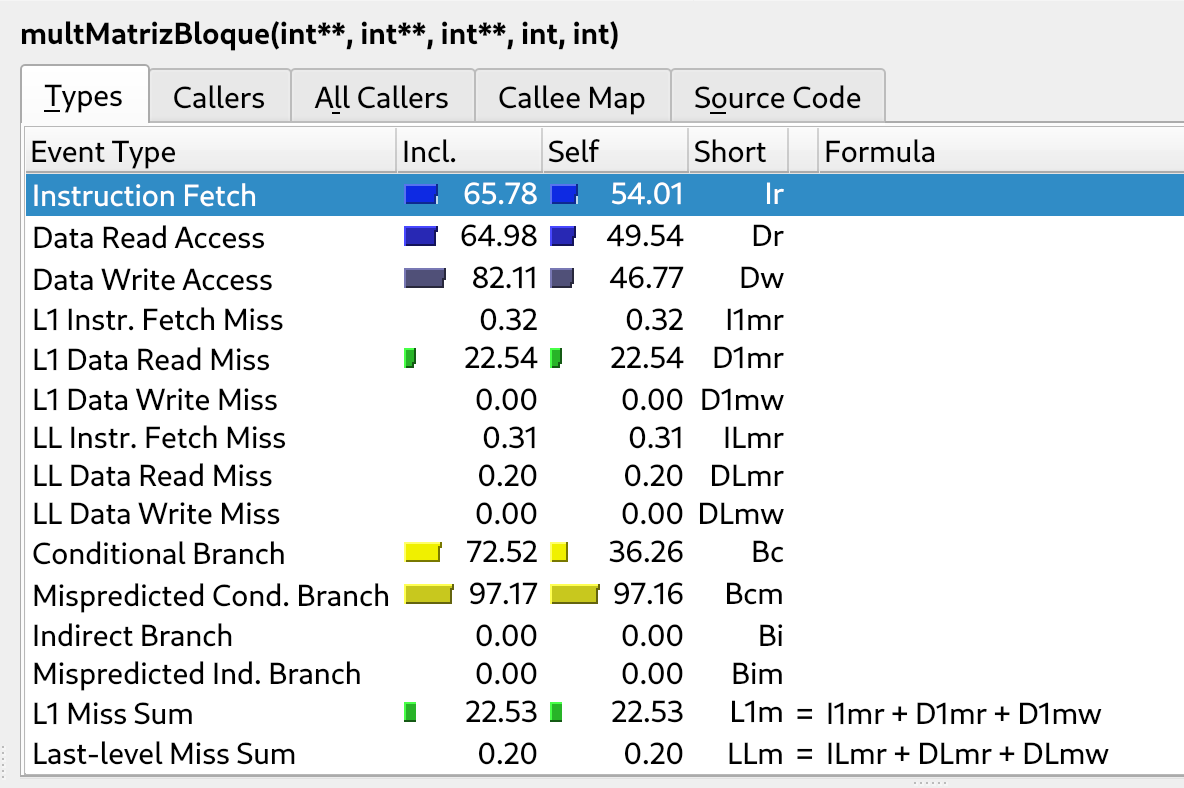
\includegraphics[width=\textwidth]{matrices_cpp_clasica.png}
            \caption{Análisis en KCacheGrind - C++ (Multiplicación lcasica)}
        \end{subfigure}
        \hfill
        \begin{subfigure}{0.45\textwidth}
            \centering
            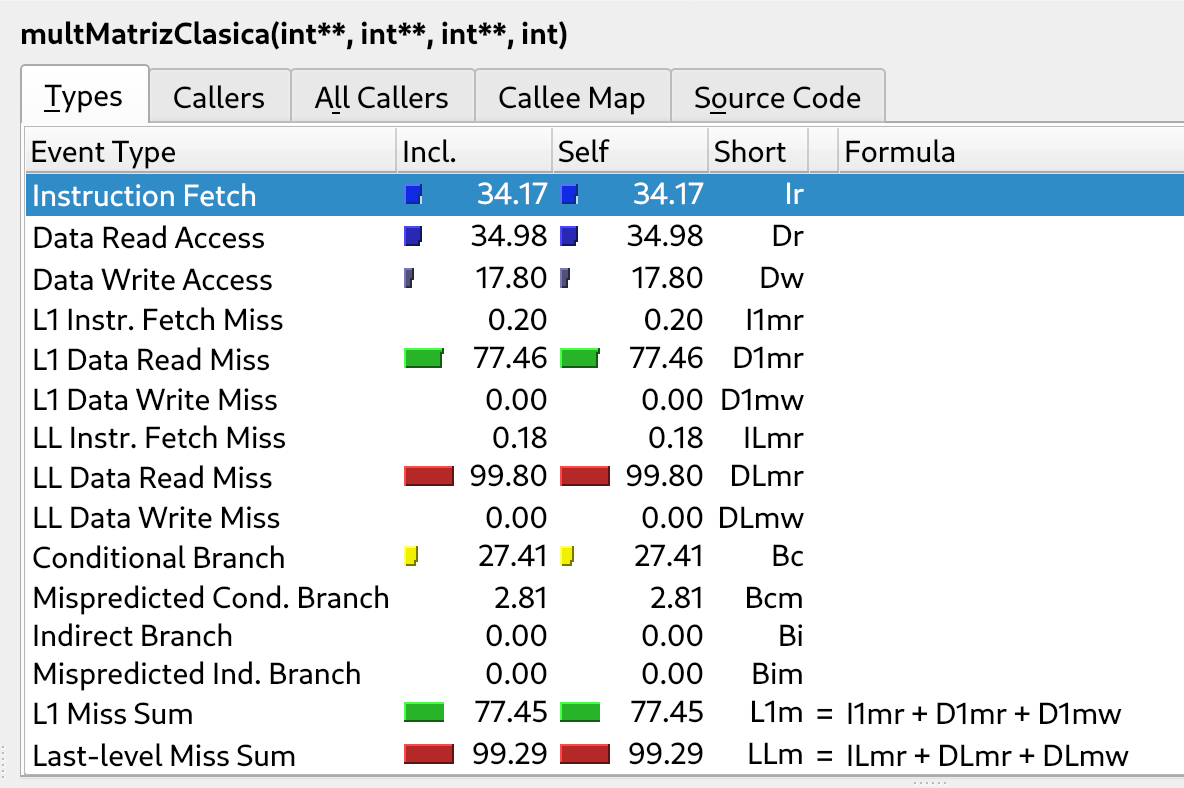
\includegraphics[width=\textwidth]{matrices_cpp_bloques.png}
            \caption{Análisis en KCacheGrind - C++ (Multiplicacion por bloques)}
        \end{subfigure}
    
        \caption{Comparación del uso de caché en C++ y Go con KCacheGrind}
        \label{fig:kcachegrindCPP2}
\end{figure}
    
La multiplicación de matrices clásica tiene una complejidad algorítmica de \(O(N^3)\), donde \(N\) es el tamaño de la matriz. Este algoritmo itera a través de cada elemento de la matriz resultante y, para cada uno, realiza una suma de productos sobre la fila de la primera matriz y la columna de la segunda matriz. Debido a su acceso a memoria en un patrón no secuencial (acceso por columnas), este enfoque puede resultar en un alto número de \textit{cache misses}, ya que los datos necesarios pueden no estar disponibles en la caché, obligando al algoritmo a acceder a la memoria principal con frecuencia.

En contraste, la multiplicación de matrices por bloques también tiene una complejidad algorítmica de \(O(N^3)\), pero su rendimiento es optimizado al dividir las matrices en submatrices o bloques. Este enfoque mejora la localidad espacial y temporal, permitiendo que los datos accedidos recientemente se mantengan en la caché por más tiempo. Durante la ejecución, los bloques se cargan en la caché, lo que minimiza la cantidad de accesos a la memoria principal y reduce significativamente el número de \textit{cache misses} en comparación con la multiplicación clásica.

Al ejecutar ambos algoritmos paso a paso, se puede observar que la multiplicación por bloques mejora el movimiento de datos entre la memoria principal y la caché. Esto se traduce en un rendimiento superior, especialmente en matrices de mayor tamaño, donde el acceso secuencial a los bloques reduce la latencia de memoria y optimiza el uso de la caché. En resumen, aunque ambos métodos tienen la misma complejidad algorítmica, la implementación por bloques ofrece una mejora considerable en la eficiencia práctica debido a un mejor manejo de la memoria caché.

\subsubsection{\textbf{Analisis con herramientas Valgrind y Kcachegrind}}


La Figura \ref{fig:kcachegrindCPP2} muestra un resumen de los resultados con una matriz de tamaño $640$, obtenidos mediante las herramientas \textit{Valgrind} y \textit{Kcachegrind}. Se observa que la multiplicación clásica de matrices presenta un elevado número de \textit{cache misses} en L1 para lectura de datos (\textbf{D1mr}), alcanzando un 77.46\%. Además, los fallos en la última caché de datos (\textbf{DLmr}) llegan al 99.80\%, lo que indica que los datos deben ser constantemente recuperados desde la memoria principal, penalizando el rendimiento del algoritmo.

En contraste, la versión optimizada por bloques mejora significativamente el aprovechamiento de la caché. Aunque la ejecución requiere un mayor número de accesos a memoria para escritura (\textbf{Dw}), la cantidad de fallos en la caché L1 es considerablemente menor, evidenciando una mejor explotación de la localidad de datos. Esto reduce la latencia causada por accesos repetidos a la memoria principal y mejora el desempeño general.

Por otro lado, la gestión de las escrituras en ambos algoritmos se mantiene eficiente, sin presentar \textit{cache misses} en la caché de escritura (\textbf{D1mw}). Esto sugiere un adecuado uso de estrategias como \textit{write-through} y \textit{write-back}, minimizando la penalización por escrituras en memoria.

En términos de predicción de saltos, la multiplicación clásica exhibe un porcentaje elevado de ramas condicionales mal predichas (\textbf{Bcm}), lo que puede causar interrupciones en el flujo de ejecución y reducir la eficiencia del pipeline del procesador. En cambio, la versión por bloques mantiene un mejor control sobre la predicción de saltos, reduciendo la penalización por cambios inesperados en el flujo del programa.

A pesar de que la multiplicación por bloques ejecuta un número mayor de instrucciones, su mejor aprovechamiento de la jerarquía de memoria compensa este costo adicional, reduciendo los \textit{cache misses} y optimizando el tiempo de ejecución.

    
\section{Conclusiones}

En el análisis del intercambio de índices para acceso a matrices, se concluye que la primera forma de acceder a los elementos por filas es significativamente más eficiente que la segunda forma, que accede por columnas. Esto se debe al mejor aprovechamiento de la localidad espacial y temporal, lo que resulta en un mayor número de \textit{cache hits} y, por ende, en un menor tiempo de ejecución.

En cuanto a la multiplicación de matrices, el uso de un algoritmo de bloques demuestra una clara ventaja en términos de eficiencia en el manejo de la caché. A pesar de ejecutar más instrucciones, su capacidad para reducir los \textit{cache misses} le permite superar a la multiplicación clásica, especialmente con matrices de gran tamaño. La optimización del uso de la memoria caché es, por lo tanto, un factor clave para mejorar el rendimiento en operaciones matriciales complejas.

\bibliography{lib}
\bibliographystyle{plainnat}


\end{document}
